\subsection{Experiment on Residue Correlation}
\label{subsec:exp:res}
\textbf{Inputs:}\\
We input a set of point clouds with the points consistently indexed respecting to their groundtruth correspondence, as shown in Figure~\ref{fig:input_for_exp_res}.\\
\begin{figure*}
	\centering
	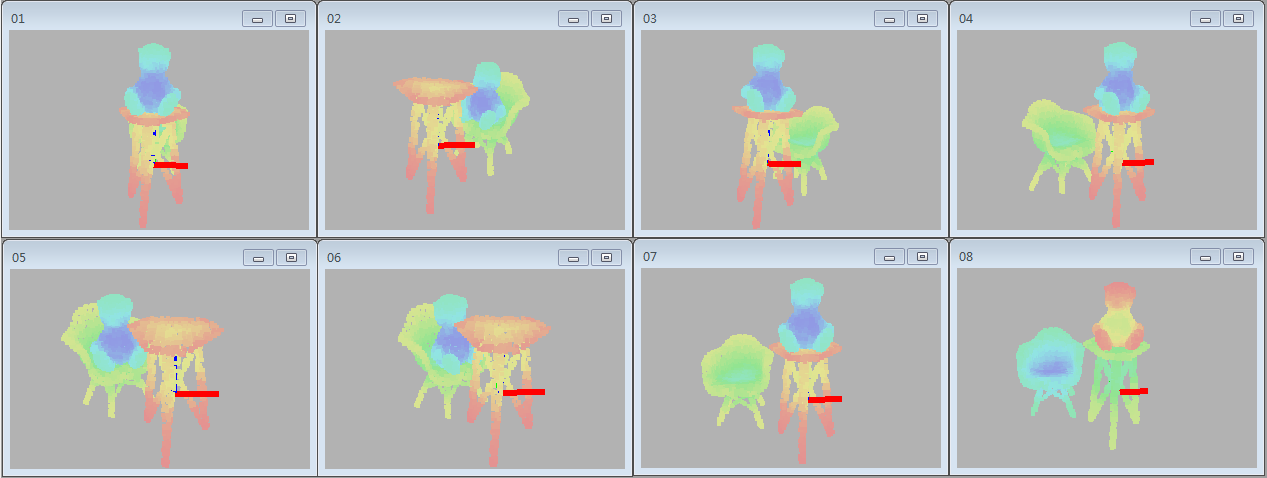
\includegraphics[width=\textwidth]{images/exp_res/inputs.png}
	\caption{Input of Experiment on Residue Correlation: The points are colored by their index. From the color you should be able to see that: In frame 01 - 07, the points are indexed consistently respecting to object in order of table, chair, teddy. In the frame 08, the points are indexed respecting to object in order of teddy, table, chair.}
	\label{fig:input_for_exp_res}
\end{figure*}
\textbf{Spectral Analysis:}\\
In order to do spectral analysis on point clouds, we first build supervoxels with \cite{Supervoxels} on point cloud and then construct a graph laplacian as a matrix $L=(a_{ij})$ defined by:
$$ a_{ij}=\left\{
\begin{aligned}
-\lambda d_{ij}-(1-\lambda) c_{ij} &~&if~i~and~j~is~an~edge\\
\sum\lambda d_{ij}+(1-\lambda) c_{ij} &~&if~i==j\\
0 &~&otherwise
\end{aligned}
\right.
$$
where $d_{ij}=\exp(\frac{-l_{ij}^2}{l_{mean}^2})$, $l_{ij}$ is the length of the edge in the graph of supervoxels and $\l_{mean}$ is average length of all edges.  $c_{ij}$ is the function indicating convexity of the edge and is defined as:
$$ c_{ij}=\left\{
\begin{aligned}
0 &~&if~\theta_{dif}<-\epsilon\\
1 &~&if~\theta_{dif}>\epsilon\\
\frac{\theta_{dif}}{2\epsilon}+\frac{1}{2} &~&otherwise
\end{aligned}
\right.
$$
where $\theta_{dif}=acos(<n_i,\frac{\overrightarrow{p_ip_j}}{||\overrightarrow{p_ip_j}||}>) - acos(<n_j,\frac{\overrightarrow{p_ip_j}}{||\overrightarrow{p_ip_j}||}>)$, in which the $\{n_i\}$ is the normal of supervoxels and $\{p_i\}$ is the center position of supervoxels.\\
Based on the laplacian matrix we can get its eigenfunctions $\{\phi_i\}_{i=0...N}$ respecting to the N smallest eigenvalues $\lambda_0...\lambda_N$.\\ 
We can also design an indicating function that maps each of the points to a unique real value. If we make this function "continue" respecting to the order of index, it can be the one shown in Figure~\ref{fig:indicating_function}   
\begin{figure*}
	\centering
	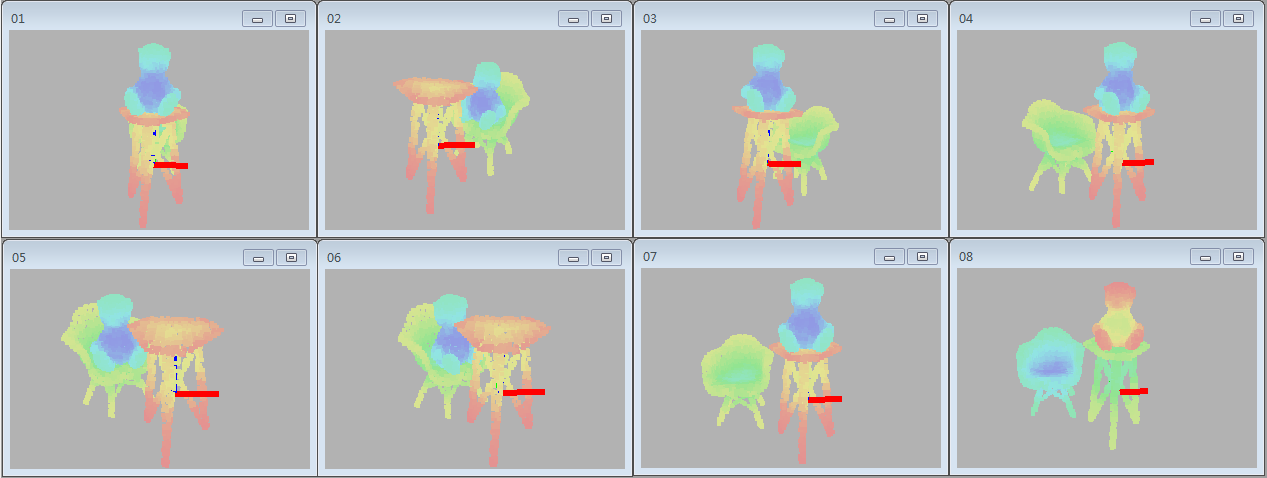
\includegraphics[width=\textwidth]{images/exp_res/inputs.png}
	\caption{Input of Experiment on Residue Correlation: The points are colored by their index. From the color you should be able to see that: In frame 01 - 07, the points are indexed consistently respecting to object in order of table, chair, teddy. In the frame 08, the points are indexed respecting to object in order of teddy, table, chair.}
	\label{fig:indicating_function}
\end{figure*}
